% !TEX TS-program = pdflatex
% !TEX encoding = UTF-8 Unicode

% Copyright (c) 2012, Edd Barrett <vext01@gmail.com>
% 
% Permission to use, copy, modify, and/or distribute this software for any
% purpose with or without fee is hereby granted, provided that the above
% copyright notice and this permission notice appear in all copies.
% 
% THE SOFTWARE IS PROVIDED "AS IS" AND THE AUTHOR DISCLAIMS ALL WARRANTIES
% WITH REGARD TO THIS SOFTWARE INCLUDING ALL IMPLIED WARRANTIES OF
% MERCHANTABILITY AND FITNESS. IN NO EVENT SHALL THE AUTHOR BE LIABLE FOR
% ANY SPECIAL, DIRECT, INDIRECT, OR CONSEQUENTIAL DAMAGES OR ANY DAMAGES
% WHATSOEVER RESULTING FROM LOSS OF USE, DATA OR PROFITS, WHETHER IN AN
% ACTION OF CONTRACT, NEGLIGENCE OR OTHER TORTIOUS ACTION, ARISING OUT OF
% OR IN CONNECTION WITH THE USE OR PERFORMANCE OF THIS SOFTWARE.

\documentclass{beamer}

\usetheme{AnnArbor}
\usecolortheme{crane}
%\usepackage{serif}
\usepackage{bytefield}
\usepackage{listings}
\usefonttheme{professionalfonts}

\title{Reversing Engineering SEGA Megadrive Games}
\author{Edd Barrett}
\date{\today}

\lstset{
  basicstyle=\ttfamily\small,
  breaklines=true,
  stringstyle=\ttfamily,
  frame=tlbr,
  framexleftmargin=1pt,
  backgroundcolor=\color{white}
}



\begin{document}



% ------------------------------

\begin{frame}[fragile]
  \titlepage
  \vspace{-4em}
  \begin{center}
  Twitter: @vext01
  \end{center}
\end{frame}

% ------------------------------

\AtBeginSection[]{%
  \begin{frame}<beamer>
    \frametitle{Outline}
    \tableofcontents[sectionstyle=show/hide,subsectionstyle=hide/show/hide]
  \end{frame}
  \addtocounter{framenumber}{-1}% If you don't want them to affect the slide number
}
\section{Intro}

\subsection{Why?}

\begin{frame}[fragile]
\frametitle{\insertsubsection}

\begin{itemize} 
\item When I was a kid I had a SEGA Megadrive (didn't we all).
\vfill
\item Since then I have learned a lot about reverse engineering.
\vfill
\item Curiosity led me to look at how these systems work.
\end{itemize}

\end{frame}

% ------------------------------

\subsection{Starting Out}
\begin{frame}[fragile]
\frametitle{\insertsubsection}

\vfill
I find the best way to learn about something is to have a clear goal.


\begin{block}{Goal 1}
\begin{center}
Sonic 3 -- Reverse the save game mechanism.
\end{center}
\end{block}

\vfill
And if I succeed:

\begin{block}{Goal 2}
\begin{center}
Make some tooling to help reverse other games too.
\end{center}
\end{block}
\end{frame}
\vfill

% ------------------------------

\section{SEGA Megadrive -- Overview}
\subsection{Basic Architcture}

\begin{frame}[fragile]
\frametitle{\insertsubsection}

A quick overview of the SEGA megadrive:

\begin{block}{CPU cores}
Basically a glorified m68k:

\begin{itemize}
\item Motorola m68000 (16MHz?)
\item Z80 (??MHz)
\end{itemize}
\end{block}

\vfill

\begin{block}{The rest}
\begin{itemize}
\item FM something XXX
\item Sq wave gen XXX
\item Custom graphics chip (VDP)
\end{itemize}
\end{block}

\end{frame}

% --------------------

\subsection{Game Cartridges}

\begin{frame}[fragile]
\frametitle{\insertsubsection}

\begin{center}
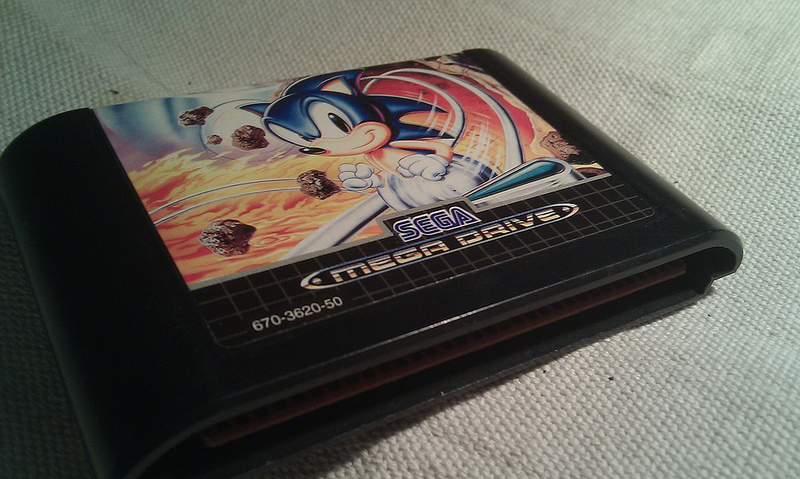
\includegraphics[height=0.8\textheight]{img/cart.jpg}
\end{center}

\end{frame}


\begin{frame}[fragile]
\frametitle{\insertsubsection}

\begin{center}
XXX INSIDE CART PIC
\end{center}

\end{frame}

% ---

\begin{frame}[fragile]

\frametitle{\insertsubsection}

\begin{block}{Inside a Typical Cart}
\begin{itemize}
\item ROM
\begin{itemize}
\item Game instructions
\item Sprites
\item Music
\end{itemize}
\vfill

\item Battery backed memory (Optional)
\begin{itemize}
\item Stores persistent state. High scores, saves etc.
\item Usually a lithium cell retain memory
\end{itemize}
\vfill

\item Additional graphics hardware (Optional)
\begin{itemize}
\item For any ``special'' graphics capabilities
\item Eg. Sega Virtua Processor
\end{itemize}
\end{itemize}
\end{block}

\end{frame}

% ------------------------------

\subsection{Memory Map of the Megadrive}

\begin{frame}[fragile]
\frametitle{\insertsubsection}

\begin{center}
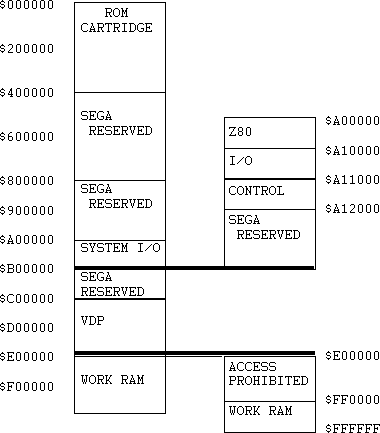
\includegraphics[height=.7\textheight]{img/mmap.png}
\end{center}
\vspace{-1em}

\begin{itemize}
\item {\small Thanks to the leaked sega2.doc we know about the memory layout.}
\end{itemize}

\footnote{Image borrowed from Nemesis}

\end{frame}

% ------------------------------

\subsection{Memory Map of a Game Cart}

\begin{frame}[fragile]
\frametitle{\insertsubsection}

XXX

\end{frame}

% ------------------------------

\section{Reversing the Sonic 3 Save RAM}

\subsection{How Do We Start -- The Electronic Engineer's Approach}

\begin{frame}[fragile]
\frametitle{\insertsubsection}

\begin{itemize}
\item Interface with Sonic 3 cart.
\item Dump save ram to disk somehow.
\item Identify field storing the level number in the save RAM.
\item Modify this field.
\item Upload modified RAM to cart.
\item Game on!
\end{itemize}

Pretty difficult and probably requires extra hardware.

\end{frame}

% ------

\subsection{How Do We Start -- The Software Engineer's Approach}
\begin{frame}[fragile]
\frametitle{\insertsubsection}

Instead:

\begin{itemize}
\item Use emulator supporting save RAM emulation (Dgen).
\item Examine on-disk save RAM dump.
\item Identify field storing the level number in the save RAM.
\item Modify save directly on disk.
\item Game on!
\end{itemize}

\vfill

Requires no special hardware or electronics knowledge :)

\end{frame}

%--------------------------------

\subsection{Bindiffing Save RAM}

\begin{frame}[fragile]
\frametitle{\insertsubsection}

\begin{itemize}
\item First we need to find the ``interesting'' parts of save RAM.
\item We can use a bindiff tool find these.
\end{itemize}

\vfill

\begin{block}{Sonic 3 Example}
\begin{itemize}
\item In emulator, start game as Sonic -- Dump save RAM
\item Now start game as Tails -- Dump save RAM
\item Bindiff the two
\end{itemize}
\end{block}

\end{frame}

%--------------------------------

\begin{frame}[fragile]
\frametitle{\insertsubsection}

XXX show outcome of bindiff.

\end{frame}

% ------

% http://www.assemblergames.com/forums/showthread.php?37200-Reverse-Engineering-The-Save-Ram-on-A-Sonic-3-Genesis-Megadrive-Cartridge

\end{document}
